%----------------------------------------------------------------------------------------
%	SLIDE 3.
%----------------------------------------------------------------------------------------
\begin{frame}
\frametitle{Implementation in Geant4 - Geometry}

\begin{exampleblock}{}
	\begin{itemize}
		\item Only simulate a $2 \times 10$ sized section of one wall of the NEBULA detector
		\item Dimensions of rods are $12\text{cm} \times 12\text{cm} \times 180\text{cm}$
	\end{itemize}
\end{exampleblock}

\begin{alertblock}{TODO}
	\begin{itemize}
		\item Assign scoring volumes to the logical volumes of the detector rods
	\end{itemize}
\end{alertblock}

\begin{figure}
	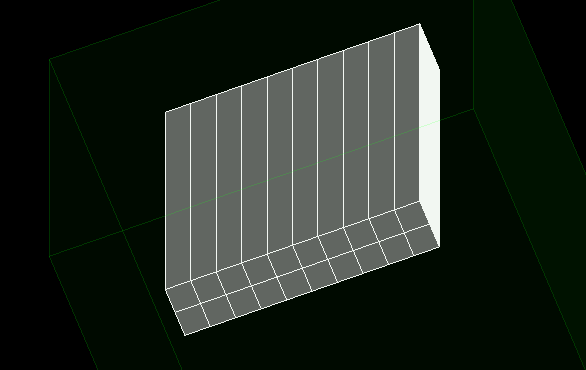
\includegraphics[width=0.5\textwidth]{images/nebula.png}
\end{figure}

\end{frame}